\documentclass[11pt]{scrartcl}
\usepackage{dominatrix}

% Graph Drawing Stuff
\usepackage{colortbl}
\usepackage{pgfplots}
\usepackage{tikz}
\usetikzlibrary{trees}
\usetikzlibrary{calc}
\pgfplotsset{compat=1.9}

% Tables
\usepackage{multirow}

% Strikeout
\usepackage{ulem}

% Jon's Name
\newcommand{\jon}{J\'{o}n }

% Additional Definitions
\newcommand{\og}{\ensuremath{\tilde{Y}}}
\newcommand{\eqname}[1]{\tag*{#1}}% Tag equation with name

\title{Fiscal Policy}
\subject{ECON W3213 Spring 2014 \jon Steinsson}
\author{Linan Qiu, lq2137}

\begin{document}

\maketitle

\begin{abstract}
This set of recitation notes introduces \textbf{Fiscal Policy}. This is in no way a substitute for attending lectures, but just in case you dozed off or checked your boyfriend's Facebook page while \jon was working Calculus magic on the board, this set of notes may save you.
\end{abstract}

\section{Fiscal Policy}

Now we're curious as to what happens when the government spends (in a deficit). We can express that as an increase in the IS curve. Recall from the previous set of notes that




\begin{figure}[H]
\begin{subfigure}[b]{0.5\textwidth}
\centering
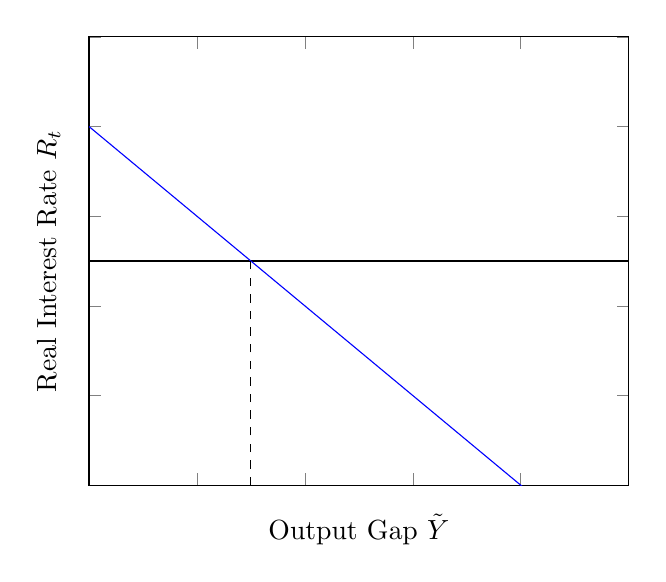
\begin{tikzpicture}
\begin{axis}[xlabel={Output Gap $\og$},ylabel={Real Interest Rate $R_t$},yticklabels={,,}, xticklabels={,,},ymin=0,ymax=10,xmin=0,xmax=10]
\addplot[black, domain=0:10]
{5};
\addplot[blue, domain=0:10]
{-x+8};
\addplot[black, domain=0:10, dashed]
coordinates{(3,0) (3,5)};
\end{axis}
\end{tikzpicture}
\caption{\color{blue}IS-\color{black}MP Diagram}
\end{subfigure}
\hspace{2ex}
\begin{subfigure}[b]{0.5\textwidth}
\centering
\begin{tikzpicture}
\begin{axis}[xlabel={Output Gap $\og$},ylabel={Inflation $\pi_t$},yticklabels={,,}, xticklabels={,,},ymin=0,ymax=10,xmin=0,xmax=10]
\addplot[black, domain=0:10]
{x};
\addplot[black, domain=0:10, dashed]
coordinates{(5,0) (5,5)};
\end{axis}
\end{tikzpicture}
\caption{Phillips Curve}
\end{subfigure}
\caption{Entire Economy}
\end{figure}

Now assume that we were originally at full employment. That's the point indicated by the dotted line.

What if we had an external shock that shifted the IS curve outwards? Then, IS shifts out. And we have a positive output gap. That will be reflected in the Phillips Curve too as we shift to a higher part of the same Phillips curve. That's what happens for this time period.

\begin{figure}[H]
\begin{subfigure}[b]{0.5\textwidth}
\centering
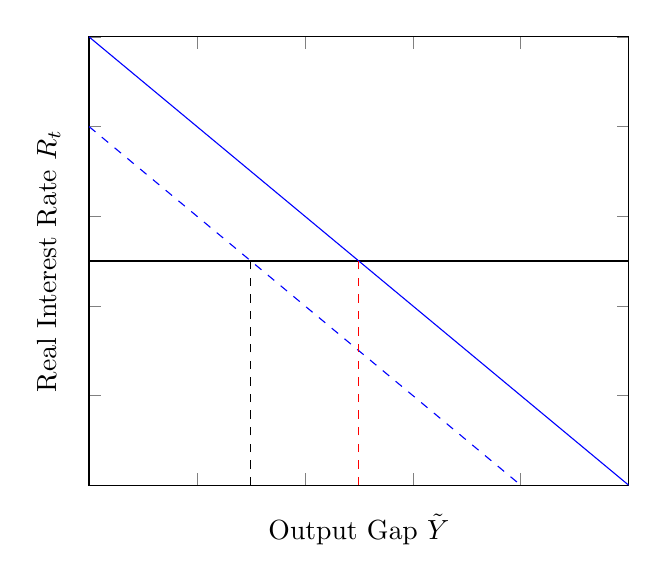
\begin{tikzpicture}
\begin{axis}[xlabel={Output Gap $\og$},ylabel={Real Interest Rate $R_t$},yticklabels={,,}, xticklabels={,,},ymin=0,ymax=10,xmin=0,xmax=10]
\addplot[black, domain=0:10]
{5};
\addplot[blue, domain=0:10, dashed]
{-x+8};
\addplot[blue, domain=0:10]
{-x+10};
\addplot[black, domain=0:10, dashed]
coordinates{(3,0) (3,5)};
\addplot[red, domain=0:10, dashed]
coordinates{(5,0) (5,5)};
\end{axis}
\end{tikzpicture}
\caption{\color{blue}IS-\color{black}MP Diagram}
\end{subfigure}
\hspace{2ex}
\begin{subfigure}[b]{0.5\textwidth}
\centering
\begin{tikzpicture}
\begin{axis}[xlabel={Output Gap $\og$},ylabel={Inflation $\pi_t$},yticklabels={,,}, xticklabels={,,},ymin=0,ymax=10,xmin=0,xmax=10]
\addplot[black, domain=0:10]
{x};
\addplot[black, domain=0:10, dashed]
coordinates{(5,0) (5,5)};
\addplot[red, domain=0:10, dashed]
coordinates{(7,0) (7,7)};
\end{axis}
\end{tikzpicture}
\caption{Phillips Curve}
\end{subfigure}
\caption{Entire Economy}
\end{figure}

Now our Phillips Curve doesn't stay constant in the next period. Nope, it shifts up because people are shmaaaaart. (or adaptive expectations. Professor Phelps please don't kill me for saying this)

\begin{figure}[H]
\begin{subfigure}[b]{0.5\textwidth}
\centering
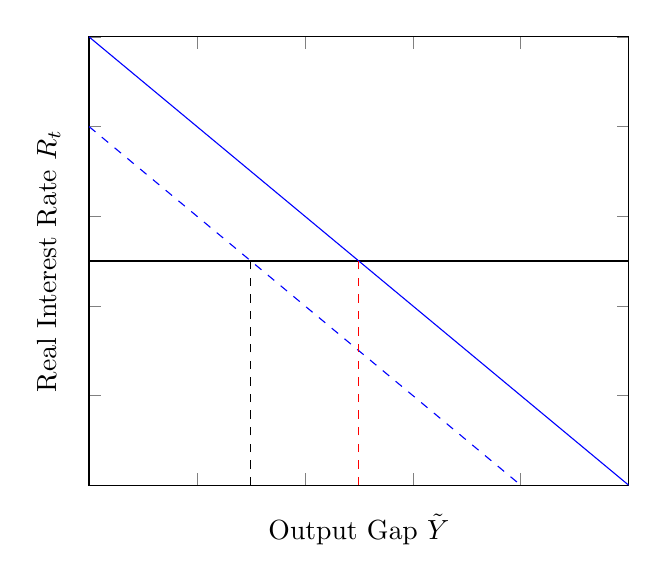
\begin{tikzpicture}
\begin{axis}[xlabel={Output Gap $\og$},ylabel={Real Interest Rate $R_t$},yticklabels={,,}, xticklabels={,,},ymin=0,ymax=10,xmin=0,xmax=10]
\addplot[black, domain=0:10]
{5};
\addplot[blue, domain=0:10, dashed]
{-x+8};
\addplot[blue, domain=0:10]
{-x+10};
\addplot[black, domain=0:10, dashed]
coordinates{(3,0) (3,5)};
\addplot[red, domain=0:10, dashed]
coordinates{(5,0) (5,5)};
\end{axis}
\end{tikzpicture}
\caption{\color{blue}IS-\color{black}MP Diagram}
\end{subfigure}
\hspace{2ex}
\begin{subfigure}[b]{0.5\textwidth}
\centering
\begin{tikzpicture}
\begin{axis}[xlabel={Output Gap $\og$},ylabel={Inflation $\pi_t$},yticklabels={,,}, xticklabels={,,},ymin=0,ymax=10,xmin=0,xmax=10]
\addplot[black, domain=0:10, dashed]
{x};
\addplot[black, domain=0:10]
{x+2};
\addplot[black, domain=0:10, dashed]
coordinates{(5,0) (5,5)};
\addplot[red, domain=0:10, dashed]
coordinates{(7,0) (7,9)};
\end{axis}
\end{tikzpicture}
\caption{Phillips Curve}
\end{subfigure}
\caption{Entire Economy}
\end{figure}

Now the central bank sees this and isn't happy. The inflation is gonna spiral out of control. So, it raises nominal interest rates, which increases real interest rates such that output gap goes back to the full employment level.

\begin{figure}[H]
\begin{subfigure}[b]{0.5\textwidth}
\centering
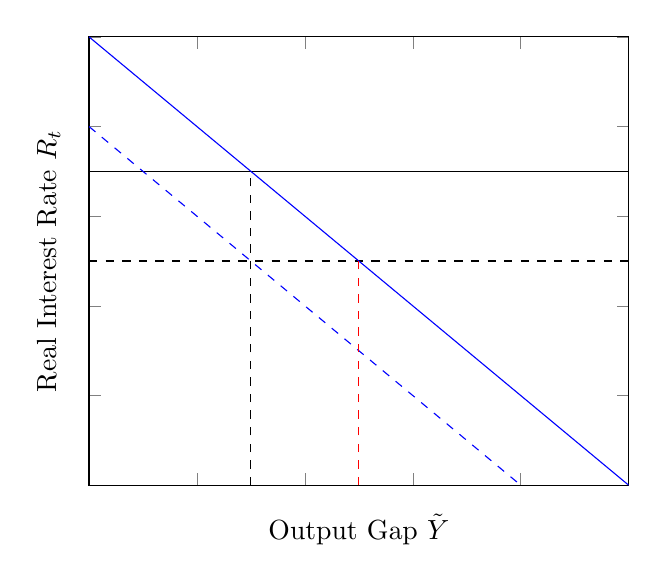
\begin{tikzpicture}
\begin{axis}[xlabel={Output Gap $\og$},ylabel={Real Interest Rate $R_t$},yticklabels={,,}, xticklabels={,,},ymin=0,ymax=10,xmin=0,xmax=10]
\addplot[black, domain=0:10, dashed]
{5};
\addplot[black, domain=0:10]
{7};
\addplot[blue, domain=0:10, dashed]
{-x+8};
\addplot[blue, domain=0:10]
{-x+10};
\addplot[black, domain=0:10, dashed]
coordinates{(3,0) (3,7)};
\addplot[red, domain=0:10, dashed]
coordinates{(5,0) (5,5)};
\end{axis}
\end{tikzpicture}
\caption{\color{blue}IS-\color{black}MP Diagram}
\end{subfigure}
\hspace{2ex}
\begin{subfigure}[b]{0.5\textwidth}
\centering
\begin{tikzpicture}
\begin{axis}[xlabel={Output Gap $\og$},ylabel={Inflation $\pi_t$},yticklabels={,,}, xticklabels={,,},ymin=0,ymax=10,xmin=0,xmax=10]
\addplot[black, domain=0:10, dashed]
{x};
\addplot[black, domain=0:10]
{x+2};
\addplot[black, domain=0:10, dashed]
coordinates{(5,0) (5,7)};
\addplot[red, domain=0:10, dashed]
coordinates{(7,0) (7,9)};
\end{axis}
\end{tikzpicture}
\caption{Phillips Curve}
\end{subfigure}
\caption{Entire Economy}
\end{figure}

Then, we first get zero output gap from our IS-MP diagram with a resulting higher real interest rate. Since we're at zero output gap, inflation stops spiraling out of control.

But here's what's interesting.

\begin{itemize}
\item Before monetary policy took place and after the IS curve shifted, we had a 1:1 increase in output gap. In other words, whatever caused the shock, say government deficit spending, it caused a proportional increase in output gap.
\item The subsequent monetary policy action removed any trace of the deficit spending.
\end{itemize}

That's what we're concerned with this time -- how much does output gap change given a certain amount of government spending. We call this the multiplier.

\begin{quote}
The fiscal multiplier is defined as the \% increase in output when government spending increases by 1\% of GDP
\end{quote}

\section{Different Multipliers}

\subsection{No Monetary Response}

We've shown that output gap increases accordingly.

Since the IS curve is given by 

\[\og_t = \bar{a} - \bar{b} (R_t -\bar{r}) \]

Then if the government increases spending by 1\% of GDP, $\bar{a}$ increases by 1\%. Given that there's no response in $R_t$, all the increases go to output gap. Hence $\og_t$ increases by 1\% as well.

\textbf{Fiscal multiplier is equal to 1}

\subsection{Monetary Response}

If monetary policy responds, we realize that the subsequent inflation will cause the central bank to act. Now going back to the IS curve,

\[\og_t = \bar{a} - \bar{b} (R_t -\bar{r}) \]

even though $\bar{a}$ increases, $R_t$ increases as well. Depending on how aggressively (remember that's given by the $\bar{m}$ variable) the central bank wants to tame inflation, the multiplier could be anything between 0 and 1. For it to be entirely zero, $R_t$ must completely offset any increases in $\bar{a}$.

\textbf{Fiscal multipler is less than 1}

\subsection{Hand to Mouth Consumer}

So far we have been assuming an IS curve that is 

\[\og_t = \bar{a} - \bar{b} (R_t -\bar{r}) \]

However, hand to mouth consumers behave differently. These are credit constrained consumers who spend temporary increases in income. Their aggregate consumption is then

\[C_t = \bar{a}'_c \bar{Y}_t +\bar{x}\og_t - \bar{b}_c \bar{Y}_t (R_t - \bar{r}) \]

where $ 0 < \bar{x} < 1$

Using the same derivation that we did for $\og_t$, we find that

\begin{align*}
\og_t &= \bar{a} + \bar{x}\og_t - \bar{b} (R_t - \bar{r})\\ 
(1-\bar{x}) \og_t &= \bar{a} - \bar{b} (R_t - \bar{r}) \\
\og_t &= \frac{1}{1-\bar{x}}[\bar{a} - \bar{b}(R_t - \bar{r})]
\end{align*}

This means that any increase in $\bar{a}$ will cause them to increase $\og_t$ by $\frac{1}{1-\bar{x}}$. The intuition is that the increase in output implies an increase in the income of these consumers. They increase their consumption, which further increases output and so on. Hence, their fiscal multiplier is larger than one.

\textbf{Fiscal multiplier is larger than 1}, specifically $\frac{1}{1-\bar{x}} > 1$

\subsection{Zero Lower Bound (Liquidity Trap)}

When a liquidity trap happens, the nominal interest rate hits 0. When that happens, the central bank no longer has power over real interest rate $R_t$ through the traditional means. Originally, 

\[ R_t = i_t - \pi_t \]

However, because $i_t = 0$,

\[ R_t = -\pi_t \]

Then, the Phillips Curve implies that 

\[ R_t = -\pi_t = -(\pi_{t-1} + \bar{v}\og_t + \bar{o}) \]

This becomes our "MP" curve on a zero lower bound or a liquidity trap. The reason why I placed quotation marks over "MP" is because it isn't really the government setting a real interest rate, hence not really monetary "policy," but rather the real interest rate moving with the central bank sitting helplessly (well actually it can do some other unconventional policies like QE).

Using the same IS curve we had earlier:

\[\og_t = \bar{a} - \bar{b} (R_t -\bar{r}) \]

Together with this new MP curve:

\[ R_t = -\pi_t = -(\pi_{t-1} + \bar{v}\og_t + \bar{o}) \]

We can plot this. Let's say that we are originally in a recession caused by a negative shock. The full employment line is the \color{red}red dashed line\color{black}. 

\begin{figure}[H]
\centering
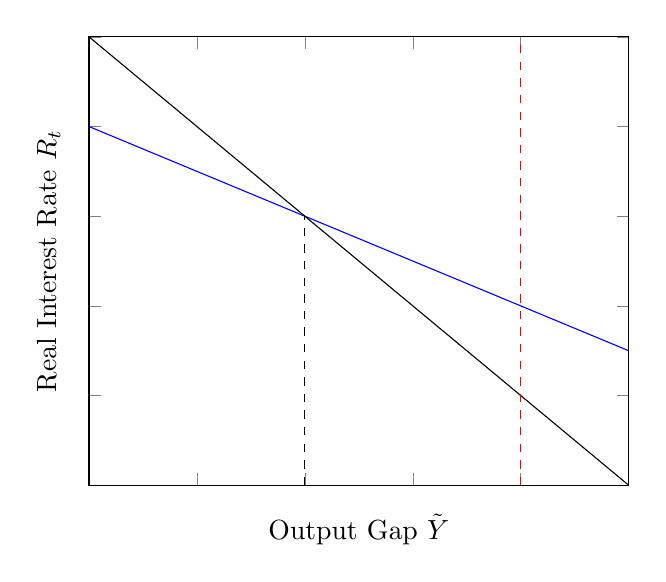
\begin{tikzpicture}
\begin{axis}[xlabel={Output Gap $\og$},ylabel={Real Interest Rate $R_t$},yticklabels={,,}, xticklabels={,,},ymin=0,ymax=10,xmin=0,xmax=10]
\addplot[blue, domain=0:10]
{-0.5*x+8};
\addplot[black, domain=0:10]
{-x+10};
\addplot[black, domain=0:10, dashed]
coordinates{(4,0) (4,6)};
\addplot[red, domain=0:10, dashed]
coordinates{(8,0) (8,10)};
\end{axis}
\end{tikzpicture}
\caption{IS-MP with Liquidity Trap (Zero Lower Bound)}
\end{figure}

What then happens is that the government can do deficit spending and shift the IS curve to the right. 

\begin{figure}[H]
\centering
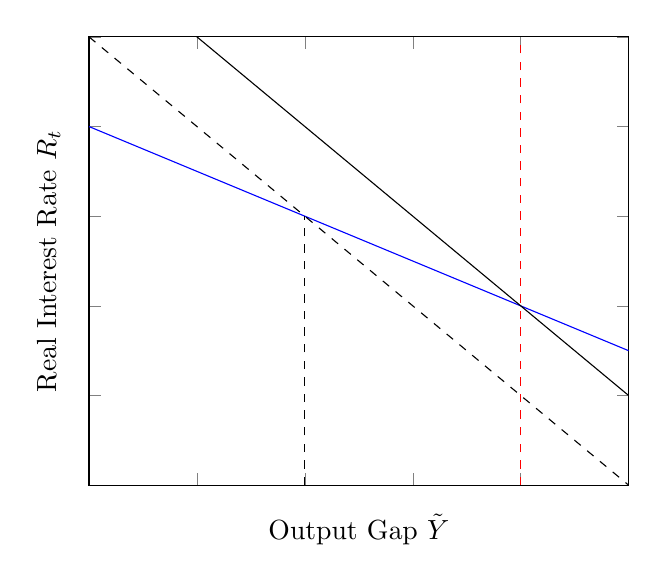
\begin{tikzpicture}
\begin{axis}[xlabel={Output Gap $\og$},ylabel={Real Interest Rate $R_t$},yticklabels={,,}, xticklabels={,,},ymin=0,ymax=10,xmin=0,xmax=10]
\addplot[blue, domain=0:10]
{-0.5*x+8};
\addplot[black, domain=0:10, dashed]
{-x+10};
\addplot[black, domain=0:10]
{-x+12};
\addplot[black, domain=0:10, dashed]
coordinates{(4,0) (4,6)};
\addplot[red, domain=0:10, dashed]
coordinates{(8,0) (8,10)};
\end{axis}
\end{tikzpicture}
\caption{IS-MP with Liquidity Trap (Zero Lower Bound)}
\end{figure}

This has shifted the output gap to the full employment level. The output gap shifted more than it would have in the case where the government had full autonomy over real interest rates $R_t$. In fact, we can do a comparison, where the blue dashed line was the original MP curve.

\begin{figure}[H]
\centering
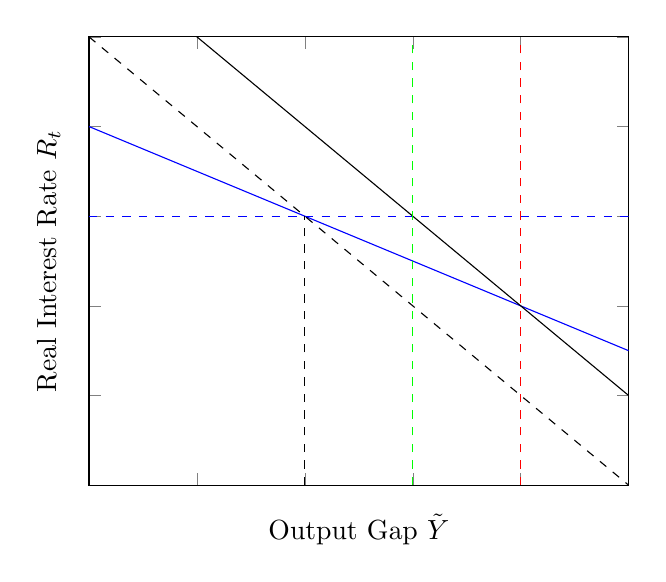
\begin{tikzpicture}
\begin{axis}[xlabel={Output Gap $\og$},ylabel={Real Interest Rate $R_t$},yticklabels={,,}, xticklabels={,,},ymin=0,ymax=10,xmin=0,xmax=10]
\addplot[blue, domain=0:10]
{-0.5*x+8};
\addplot[blue, domain=0:10,dashed]
{6};
\addplot[black, domain=0:10, dashed]
{-x+10};
\addplot[black, domain=0:10]
{-x+12};
\addplot[black, domain=0:10, dashed]
coordinates{(4,0) (4,6)};
\addplot[green, domain=0:10, dashed]
coordinates{(6,0) (6,10)};
\addplot[red, domain=0:10, dashed]
coordinates{(8,0) (8,10)};
\end{axis}
\end{tikzpicture}
\caption{IS-MP with Liquidity Trap (Zero Lower Bound)}
\end{figure}

In fact, if we were using the original MP curve, we would only hit the green dashed line. Hence, we conclude that the fiscal multiplier is larger than 1.

To recap, the government increases spending by 1\% of GDP. This higher output gap raises inflation and lowers real interest rate which further increases output. We have combined all these effects into the modified MP curve (that's downward sloping since increases in output gap raises inflation, lowers real interest rate). This is kind of like a \emph{virtuous spiral}.

\textbf{Fiscal multiplier is larger than 1}

\subsection{Wasteful vs Useful Spending}

Finally, we add the case that if government spending was useful, then you would not be motivated to work additionally to purchase more goods (since the government would do that for you).

\textbf{Fiscal multiplier is 0}

However, if the government wasted the money on wars in the Middle East, you'd have to spend additional money on healthcare, education etc. Hence, you'd work more.

\textbf{Fiscal multiplier is than between 0 and 1}

\jon provided lots of evidence for both cases (that's pretty much the last lecture), so I shan't repeat them here.



\end{document}